\documentclass[12pt,a4paper]{article}
\usepackage[utf8]{inputenc}
\usepackage{fullpage}

\usepackage{graphicx}
\graphicspath{ {./Screenshots/} }

\title{CMPE 230 - Project 3 Documentation}
\author{Karahan Sarıtaş (2018400174) \\ Cahid Arda Öz (2019400132)}

\begin{document}

\maketitle

\tableofcontents

\section{Problem Statement}

We are asked to develop a QT program that displays conversion rate information about crypto-currencies. We extract the information from an API designed by coingecko.\par

\section{Solution}

Our solution consists of Main function and DataExtractor class. Within Main, we create our QT objects such as grid layout and main window widget. Then we create a DataExtractor object. 
DataExtractor reads a file consisting of the list of crypto currencies that will be displayed. It obtains the name of the file from an environment variable named MYCRYPTOCONVERT. \par
Then DataExtractor sends network requests to the API and receives information. We wait for each request to complete receiving a reply before continuing our procedure. Once a request has received its reply, DataExtractor stores the related information in a QString and proceeds with the next task.\par
After getting information from DataExtractor, we parse it within the Main function with the help of QRegularExpression and store the currencies in vectors. Then we create a grid and set the horizontal and vertical labels accordingly. \par
Lastly, we add numerical values to the grid and add the grid layout to the main window, completing the procedure. \par

\section{Implementation}

Our implementation consists of a main function in which we parse the information and create our grid, and a DataExtractor object that makes the http request to get currency-rate information. \par

\begin{enumerate}
 \item Main Function
 \item DataExtractor
\end{enumerate}

We used necessary standard libraries and QT libraries such as QGridLayout, QApplication, QLabel, QStringList, QString, QtNetwork, QUrl and QRegularExpression. \par
First, within Main function we generate a QWidget,and QGridLayout. We create a DataExtractor object to get the currency-rate information. Using regular expressions, we parse the information QString into cryptos and corresponding currency values. After storing them in vectors, we fill the rows, columns and labels of the grid. Then we add the grid layout to the main window. \par


\subsection{Data Extraction}

As stated above, DataExtractor object is responsible for both reading the file obtained from environment variable MYCRYPTOCONVERT and sending the network requests to the API. \par
DataExtractor consists of a constructor, destructor, public slots and private fields. Public slots are namely replyFinished(), CoinsList(), getData() and getCryptos(). Private fields are two QNetworkAccessManager pointers, a vector of strings named as cryptos, and two QString objects to store the crypto-currencies and list of coins respectively. \par

\begin{enumerate}
    \item DataExtractor(std::string os, QWidget *parent = 0): This is the constructor of DataExtractor object. It takes a string that represents the operating system. We get the information as to the OS within the main function and then create a DataExtractor object. Within the constructor, we also read the file that contains a list of crypto-currencies. Then two network requests are sent to the API and we wait for the responses. First request aims to fetch the list of coins available at coingecko. Second  request aims to gather currency-rate information for necessary crypto-currencies. After receiving the responses, we store the information in strings, which are private fields of our object. Basically, constructor performs all important tasks for the extractor object. 
    \item DataExtractor::replyFinished(QNetworkReply *reply): This method stores the result of our second network request (crypto-currency rate information) to a string.
    \item DataExtractor::CoinsList(QNetworkReply *reply): This method stores the result of our first network request (coins list) to a string.
    \item QString DataExtractor::getData(): Getter function that returns the data received from the API.
    \item std::vector\textless std::string\textgreater DataExtractor::getCryptos(): Getter function that returns the list of crypto-currencies to be displayed in the grid.
    \item DataExtractor::~DataExtractor(): Destructor deletes the QNetworkManager pointer to avoid memory leaks. 
\end{enumerate}

\subsection{Regular Expression}

Within Main function, we parse the information received from the API by using QRegularExpressions. We used two different regular expressions to capture the crypto pattern (including the currency rate information), and to capture the currency pattern respectively. 
\begin{enumerate}
    \item cryptoPattern: \verb|"\"([\\w-]+)\":{([^}]*)}"|
    \item currencyPattern: \verb|"\"([\\w-]+)\":(\\d+\\.?(e-?)?\\d*),?"|
\end{enumerate}

After the parsing procedure is complete, we store the tokens in a 2D vector. Each row of the vector represent the currency information for one crypto-currency. Order of the crypto-currencies is the same with the order of crypto-currencies stored in the currency vector returned by the DataExtractor. \par
After storing the results we proceed with the next step, creating a grid with appropriate width and height settings. \par

\subsection{Grid Generation}

To generate the grid layout, we iterate through our currency and crypto lists. Once the labeling is done, we can proceed with inserting data to the grid. To do so, we simply iterate through our 2D vector and fill the cells of the grid layout. Then we set minimum width and minimum height for columns and rows respectively.  \par
Lastly, we add our grid layout to the main window by using .setLayout() method. \par

\section{Examples}

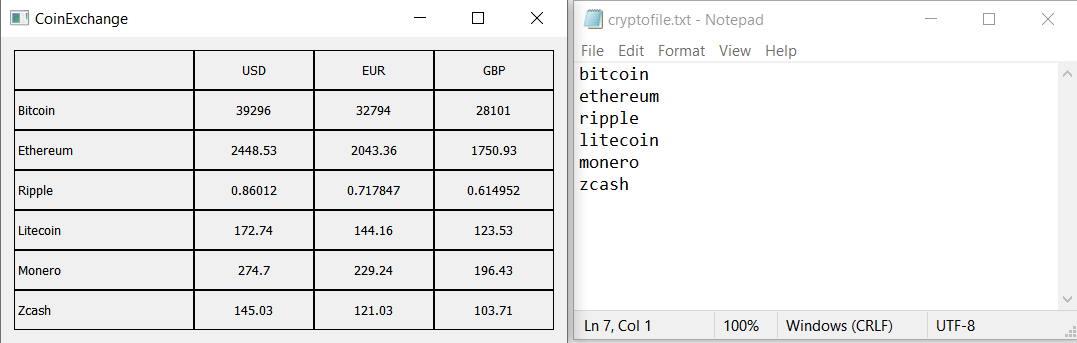
\includegraphics[width=15cm]{Table1.png} \par
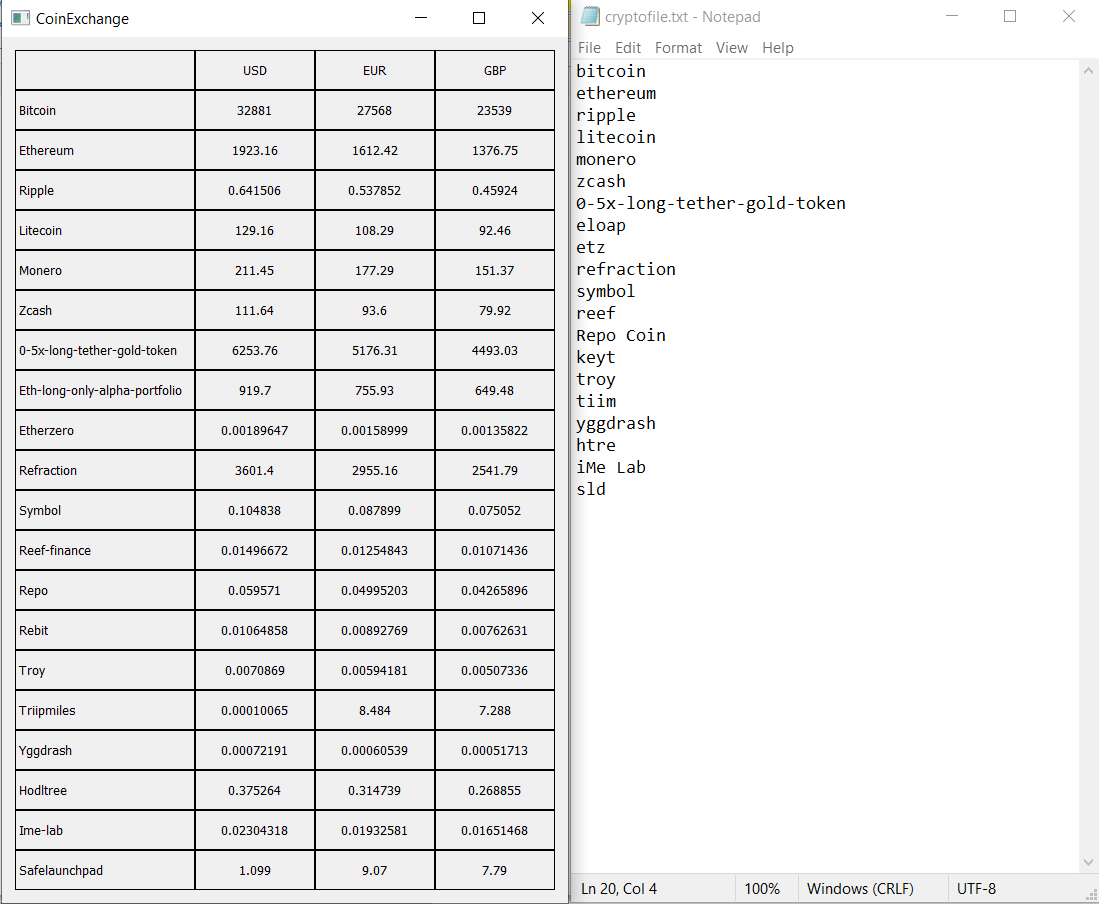
\includegraphics[width=15cm]{Table2.png}

\section{Conclusion}

Looking at the visual material we get at the end, we conclude that our program solves the given problem. We extracted the information correctly and generated a QT grid as stated in the description.

\end{document}